\documentclass[10pt]{article}

% Les packages
\usepackage[french]{babel} \usepackage[utf8]{inputenc}
\usepackage[T1]{fontenc} \usepackage[top=3.5cm, bottom=3.5cm, right=3cm,
  left=3cm]{geometry} \usepackage{amsmath} \usepackage{amssymb}
\usepackage[table]{xcolor}
\usepackage[colorlinks]{hyperref} % Pour les liens du sommaire cliquables.
\usepackage{graphicx}
\usepackage{float}
\usepackage[french,linesnumbered]{algorithm2e}
\usepackage{listings}
\usepackage{multicol}
\usepackage{tikz}
\usepackage{color}

\begin{document}
% Mise en place de la page de garde.
  \begin{titlepage}
    ~ \vfill
    \begin{center}
      \LARGE ENSEIRB-MATMECA\\ \LARGE Filière Informatique\\[1.5 cm]

      {\Large \bfseries \bsc{--- Projet de SGBD ---}}\\[0.5 cm]

      \rule{\linewidth}{0.5 mm}\\[0.4 cm] {\Huge \bfseries Gestion d'une flotte de vélos électriques\\[0.2 cm]} \rule{\linewidth}{0.5 mm}\\[1.5 cm] {\Large
      Hugo \bsc{Langlais} \quad Antoine \bsc{Gaudy} \quad Guillaume \bsc{Fornes} \\[0.5 cm]}

      {\large Encadré par Sylvain \bsc{Lombardy}}\\ \vfill
      
\includegraphics[scale=0.4]{img/logo.em-bxinp} \vfill
      {\large Semestre 7 - 2021}
    \end{center}
  \end{titlepage}

  \tableofcontents
  \newpage

  \section{Introduction}\label{sec:intro}
  \section{Modélisation des données}\label{sec:modelisation}
  Afin d'élaborer un système de gestion base de données permettant de répondre au problème, nous devons dans un premier temps
  comprendre les besoins du client afin de modéliser par la suite un modèle entité association de la base que nous souhaitons créer.\\

  \subsection{Contexte de la base de donnée}\label{subsec:contexte}
  Les systèmes de vélos empruntables momentanément pour un trajet ou plus se multiplient.
  Ces systèmes sont appréciés en ville, car ils permettent au client d'éviter d'avoir à acheter un vélo et résolvent le problème
  de la nécessitée d'un emplacement de stockage personnel de ce dernier. \\
  Notre client désire ici developer son propre système de location de vélos électriques et souhaite donc mettre en place une base de
  donnée afin de gérer ce dernier.
  L'objectif est donc de pouvoir gérer une quantité de vélo, d'adhérents ainsi que les différentes stations des différentes communes
  concernées par le système.
  De plus il faudra pouvoir modéliser et répertorier les différents emprunts, ceci concernant donc un vélo, son utilisateur adhérent au système,
  le temps de trajet et le kilométrage effectué.\\

  \subsection{Modèle entité-association}\label{subsec:modele}
  Une fois le contexte étudier, il nous faut analyser les différentes opérations que désire pouvoir effectuer notre client.
  Elles aideront à définir notre schéma d'entité association, car le système devra s'assurer de la possibilité de leur réalisation.
  Celles-ci seront définies comme des requêtes dans notre base, séparées en deux types.\\
  D'une part, nous aurons des requêtes de consultation, permettant d'obtenir des informations sur les vélos, stations, adhérents\dots
  De plus le client désire pouvoir lister les vélos par station, ceux en cours d'utilisation, les stations dans une commune,
  ou encore la liste des adhérents ayant emprunté au moins deux vélos différents dans une journée.
  Elles nous permettent d'établir les relations nécessaires entre les différentes tables, ainsi que des informations sur les attributs de ces dernières\\
  D'autre part, il devra y avoir de requêtes de statistiques, notamment sur la moyenne du nombre d'usagers par vélo par jours,
  la moyenne des distances parcourues par les vélos par semaine, le classement des stations par nombre de places disponibles pour
  une commune, et enfin le classement des vélos par charges de batterie pour une station donnée.\\

  Hormis la consultation d'informations générales sur certaines entités, La majorité de ces requêtes concerne les emprunts effectués.
  Ainsi la position de l'entité des emprunts se dessine comme centrale dans la base de donnée
  \begin{figure}[!h]
    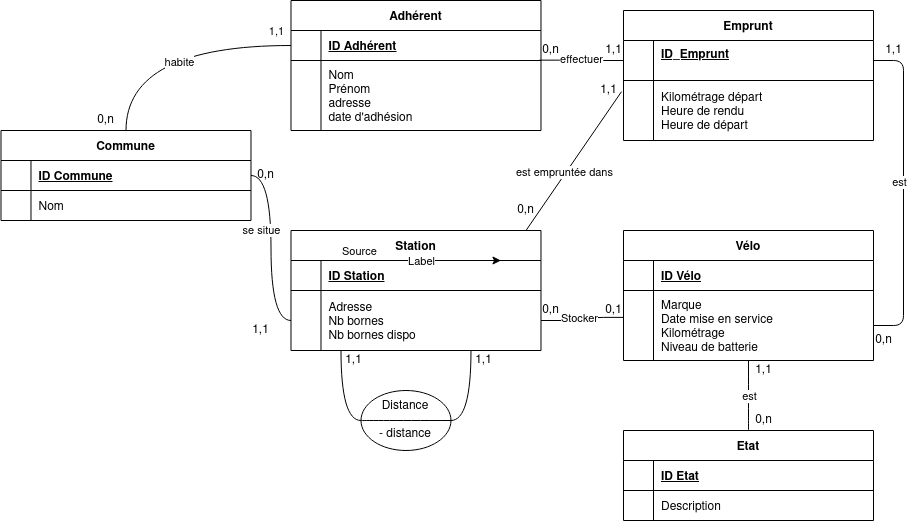
\includegraphics[scale=0.5]{img/entite_association}
    \caption{Schéma entité-association}
    \label{entite}
  \end{figure}
  \section{Schéma relationnel}\label{sec:relationel}
  \subsection{Schéma en 3e forme normale}\label{subsec:normal}

  \subsection{Contraintes et dépendances}\label{subsec:contrainte}

  \section{Implémentation}\label{sec:implementation}
  \subsection{Création et remplissage de la base de donnée}\label{subsec:crea}
  \subsubsection{Les tables}
  \subsubsection{Les Triggers}
  \subsubsection{Les procédures}
  
  \subsection{Implémentation des requêtes}\label{subsec:requete}
  \subsubsection{Les consultations}
  \subsubsection{Les statistiques}
  
  \section{Utilisation}\label{sec:utili}
  \subsubsection{Description du \textit{front}}\label{subsec:desc}
  \subsubsection{Possibilité et utilisations}\label{subsec:possib}

  \section{Conclusion}\label{sec:ccl}
\end{document}